\chapter{Introduction\label{sec:intro}}

%Standard Model
% - What does it consist of (particles, interactions, gauge fields)
% - Description of Higgs mechanism and its significance
% - Examples of SM limitations (DM, gravity, Higgs loop corrections...)

%Supersymmetry
% - What is supersymmetry, what SM problems does it address
% - 2HDM, NMSSM: Motivations
% - 

\subsection{The Standard Model\label{sec:SM}}

The Standard Model is a quantum field theory that provides the most successful description to date of all experimentally observed fundamental particles and their interactions. In this framework, the fundamental particles are all treated as excitations of quantum fields, and interactions between particles occur via the exchange of mediating particles~\cite{BettiniPhysics}.
Fundamental particles can be classified into three main categories: leptons, quarks, and gauge bosons. The leptons and quarks are all fermions -- particles with half-integer spin whose dynamics obey the Dirac equation. Leptons have integer electric charge and fall into three categories called ``flavours", each of which can be regarded as a representation of the SU(2)xU(1) group. The negatively charged leptons are the electron, the muon, and the tau (in increasing order of mass), and each is associated with a massless neutrino; for each lepton, there is also an associated antiparticle. Quarks have fractional electric charge and fall into three categories known as ``colour", which can be regarded as representations of the SU(3) group.
Particles interact via four fundamental forces: the strong force, electromagnetism, the weak force, and gravity. These interactions are mediated by the third category of fundamental particle, the gauge bosons. The strong force is mediated by gluons, which are colorless, electrically neutral, and massless; only quarks and gluons can participate in strong interactions. Any charged particle can participate in electromagnetic interactions, which are mediated by colorless, electrically, neutral, massless photons. The weak force, which is responsible for nuclear decays, is mediated by the W bosons, which can have positive or negative charge, and Z bosons, which are electrically neutral.
An illustration of the classification of Standard Model particles is shown in Fig.~\ref{fig:StandardModelTable}.

\begin{figure}
   \begin{center}
      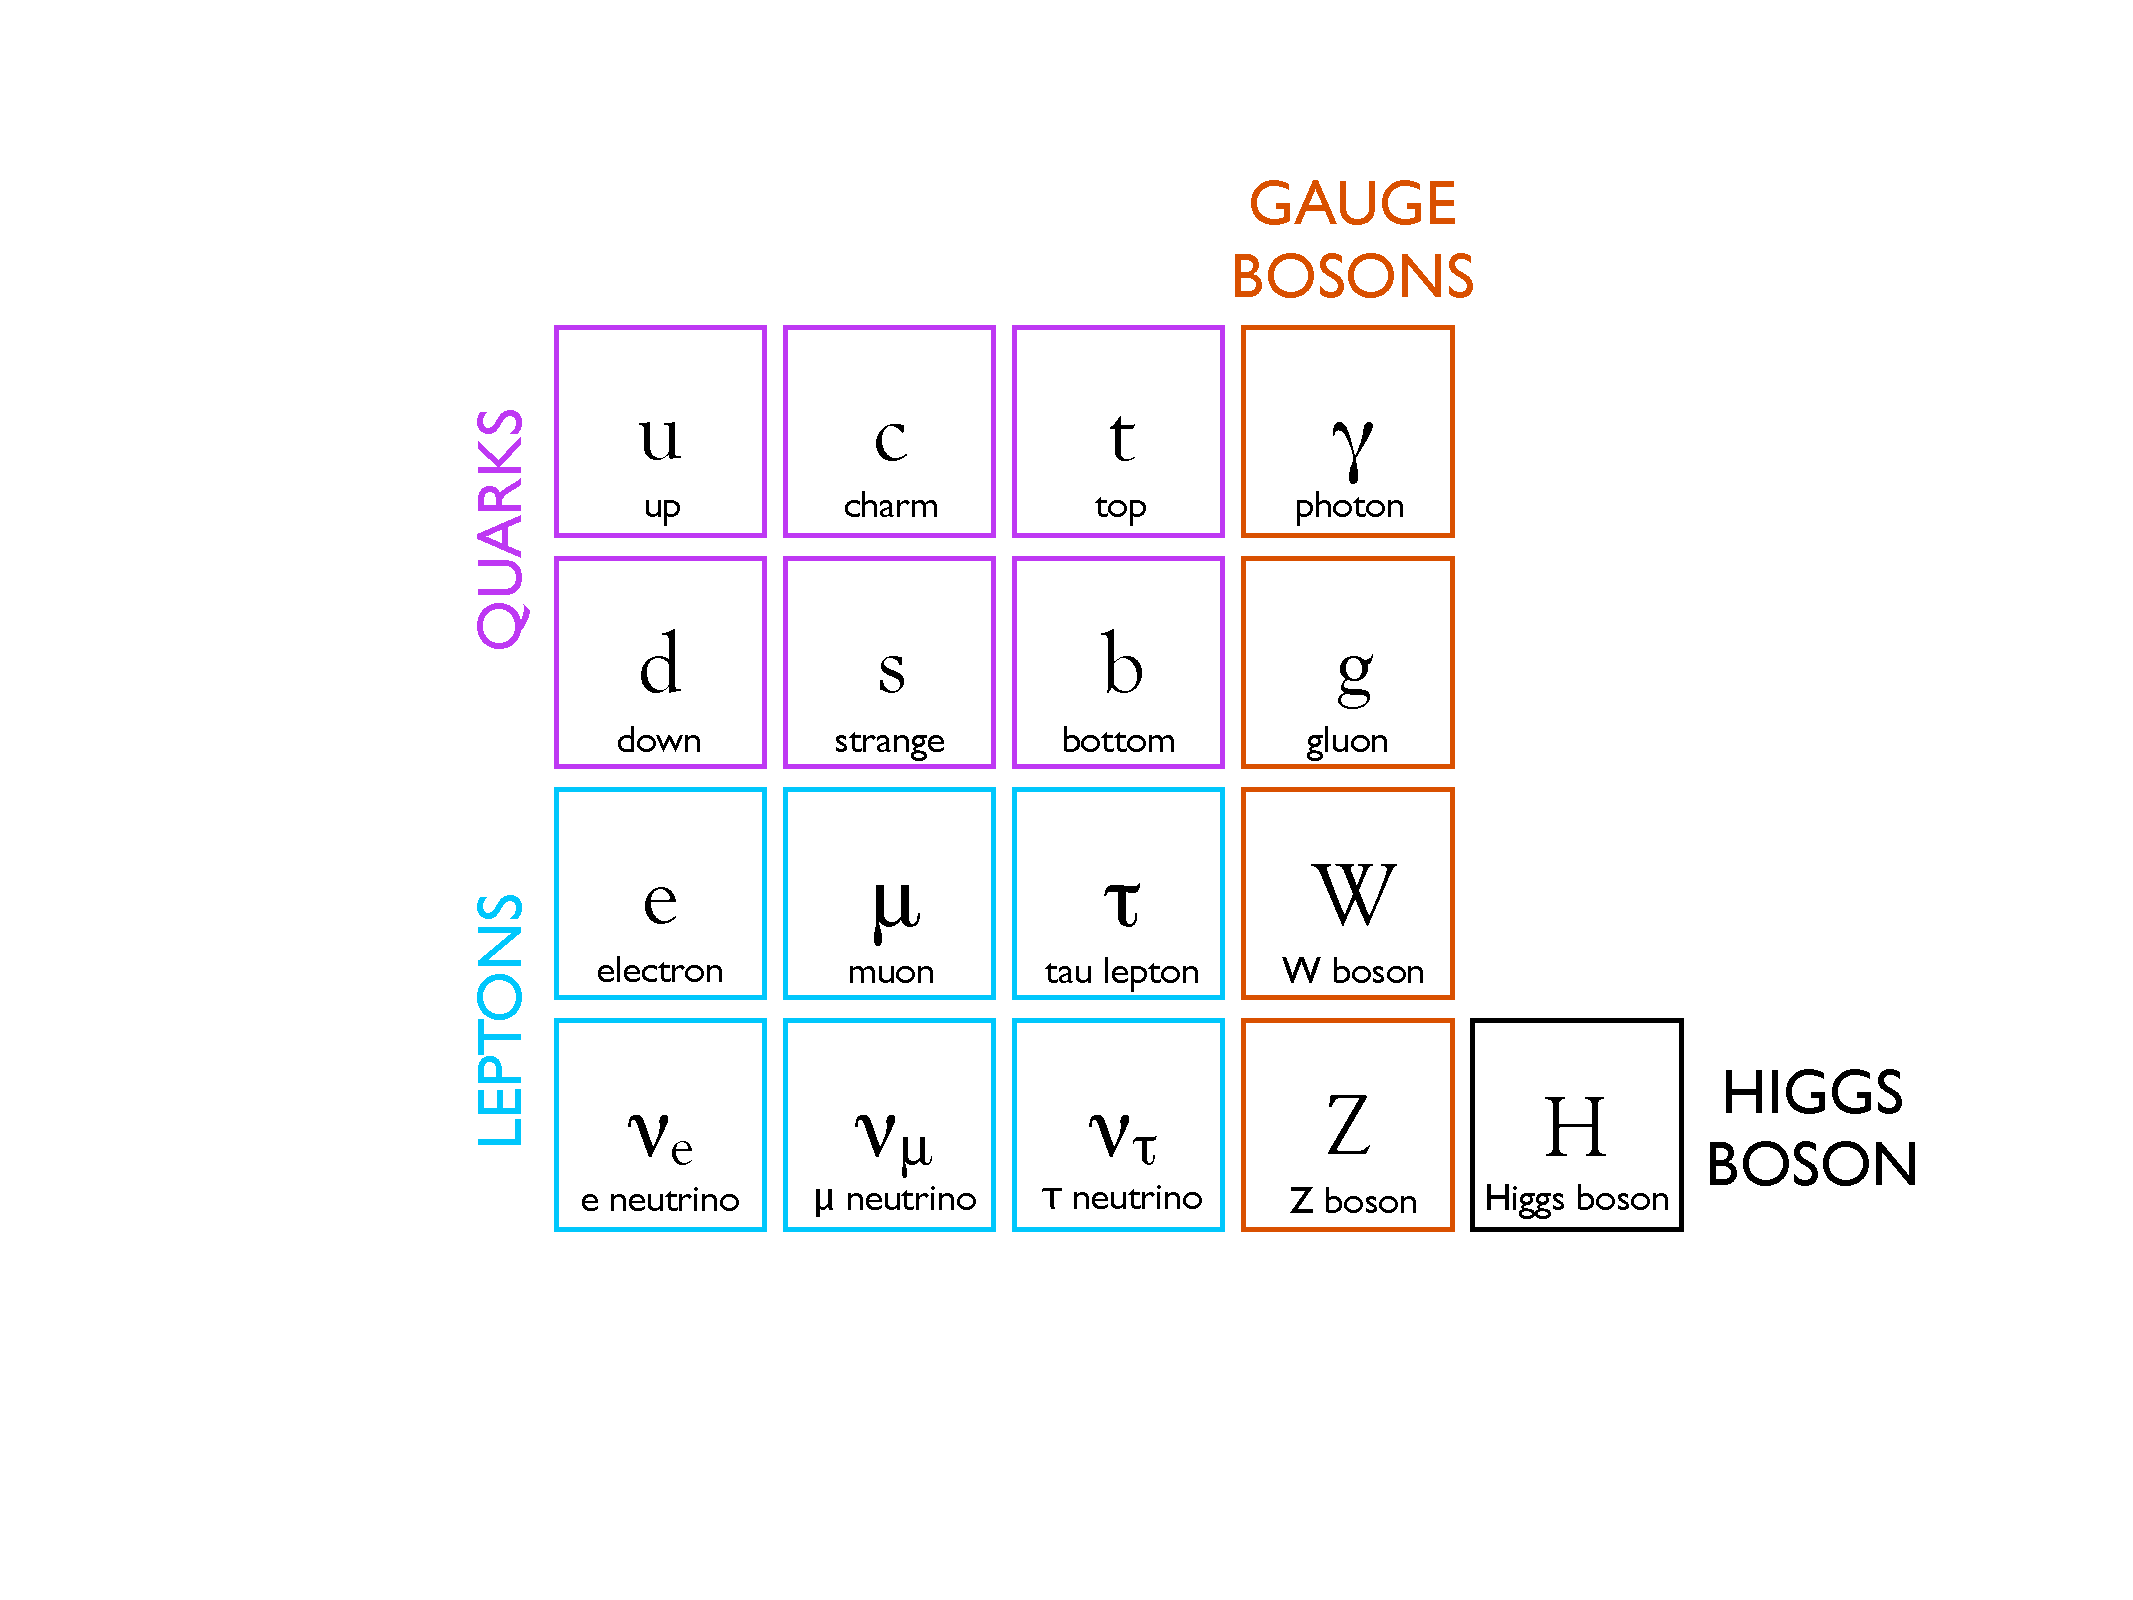
\includegraphics[width=0.4\textwidth]{figures/StandardModelTable}
      \caption{Standard Model particles.}
      \label{fig:StandardModelTable}
   \end{center}
\end{figure}

\subsection{Deficiencies of the Standard Model\label{sec:SMdeficiencies}}

Although the Standard Model has been successful in describing a wide range of experimental results, it also falls short of providing a complete description of nature in many respects. It describes only three out of the four fundamental forces; the way in which gravity, which is $10^{-32}$ times weaker than the weak force, factors into the Standard Model is still unknown. It fails to provide a satisfactory description of neutrino oscillations, an explanation of the matter-antimatter asymmetry in the universe, or a suitable candidate (or candidates) for dark matter.

The Standard Model also predicts that the mass of the Higgs boson receives loop corrections -- corrections of a magnitude close to the Planck scale at which the three fundamental forces are expected to be unified. The fact that the experimentally measured Higgs boson mass is 125 GeV -- orders of magnitude smaller than the corrections -- means that these loop corrections must somehow be cancelled, but it is not known how. This constitutes what is known as the hierarchy problem of particle physics.

\subsection{Supersymmetry}

One theory that has been proposed to address the hierarchy problem is that there exists a certain symmetry, referred to a supersymmetry, that relates fermions to bosons. For each fermion, there would exist a corresponding bosonic parter particle, and likewise for each boson there would exist a fermionic partner; under a supersymmetric transformation, a fermion would turn into its bosonic partner and vice versa. Thus, for each loop correction to the Higgs mass, there would be another loop correction from the supersymmetric partner particle; since fermionic loops have a sign opposite that of bosonic loops, the loop corrections would cancel neatly.

\subsubsection{MSSM}

\subsubsection{NMSSM}
